\newpage
\section{Diagrama de clases}
Un diagrama de clases sirve para representar gráficamente la estructura de un sistema cuya implementación se llevará a cabo mediante un lenguaje de programación orientado a objetos. Dentro de la etapa de diseño y posterior al análisis de requerimientos es que se realiza el diagrama de clases para el sistema. El principal objetivo de estos diagramas es representar las clases y su contenido, así como su relación con otras clases \cite{clases}.

\subsection{Componentes de un diagrama de clases}
A continuación se describirán los componentes de un diagrama de clases, estos componentes se encuentran dentro del Lenguaje Unificado de Modelado (Unified Modeling Language, UML\footnote{\url{https://www.uml.org/}} por sus siglas en ingles)\footnote{De aquí en adelante se empleará UML para referirse al Lenguaje Unificado de Modelado}.

\begin{itemize}
	\item \textbf{Clase}: Es el componente básico para el diagrma de clases, estas representan las entidades o conceptos. Dentro de las clases se definen los atributos y métodos que utilizarán los objetos de la clase. La Figura \ref{fig:clase} muestra un ejemplo de como se representa una clase.
	
	\hypertarget{fig:clase}{
		\begin{figure}[htbp]
			\begin{center}
				\hypertarget{fig:clase}{
					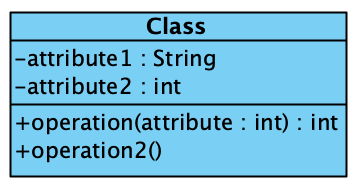
\includegraphics[ scale=.8]{analisisRequerimientos/clases/images/clase}
					\caption{Ejemplo de clase}
				}
				\label{fig:clase}
			\end{center}
		\end{figure}
	}

	\item \textbf{Atributos y métodos}: Los atributos generalmente se muestran sus nombres y con su tipo, mientras que los métodos además de su nombre se incluye su tipo de retorno, en caso de que tenga, y los parámetros de entrada que recibe. Así mismo, tanto atributos como métodos están acompañados de un símbolo antes de su nombre, estos símbolos representan:
	
	\begin{itemize}
		\item \textbf{+} representa atributos públicos.
		\item \textbf{-} representa atributos privados.
		\item \textbf{\#} representa atributos protegidos.
	\end{itemize}

	\item \textbf{Relaciones}: Ya que las clases se relacionan entre sí, existen distintos tipos de relaciones:
	
	\begin{itemize}
		\item \textbf{Generalización}: Representa una extensión o herencia de una clase de otra. La Figura \ref{fig:generalizacion} muestra un ejemplo de esta relación.
		
		\hypertarget{fig:generalizacion}{
			\begin{figure}[htbp]
				\begin{center}
					\hypertarget{fig:generalizacion}{
						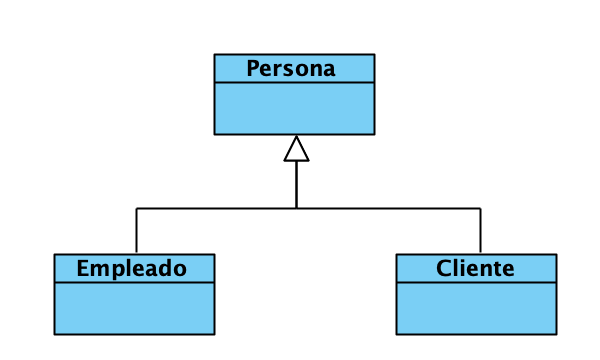
\includegraphics[ scale=.8]{analisisRequerimientos/clases/images/generalizacion}
						\caption{Ejemplo de generalizacion}
					}
					\label{fig:generalizacion}
				\end{center}
			\end{figure}
		}
		
		\newpage
		\item \textbf{Asociación}: Es una relación básica entre dos clases. Pueden ser unidireccionales (Figura \ref{fig:unidireccional}) o bidireccional (Figura \ref{fig:bidireccional}). 
		
		\hypertarget{fig:unidireccional}{
			\begin{figure}[htbp]
				\begin{center}
					\hypertarget{fig:unidireccional}{
						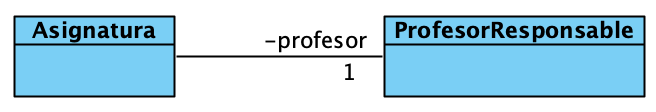
\includegraphics[ scale=.8]{analisisRequerimientos/clases/images/unidireccional}
						\caption{Ejemplo de unidireccional}
					}
					\label{fig:unidireccional}
				\end{center}
			\end{figure}
		}
		
		\hypertarget{fig:bidireccional}{
			\begin{figure}[htbp]
				\begin{center}
					\hypertarget{fig:bidireccional}{
						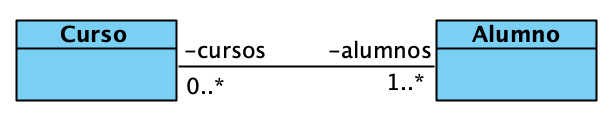
\includegraphics[ scale=.8]{analisisRequerimientos/clases/images/bidireccional}
						\caption{Ejemplo de bidireccional}
					}
					\label{fig:bidireccional}
				\end{center}
			\end{figure}
		}
	
		\item \textbf{Agregación}: Representa que un objeto de una clase contiene objetos de otra clase. La Figura \ref{fig:agragacion} muestra un ejemplo de una agregación.
		
		\hypertarget{fig:agragacion}{
			\begin{figure}[htbp]
				\begin{center}
					\hypertarget{fig:agragacion}{
						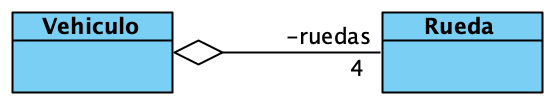
\includegraphics[ scale=.8]{analisisRequerimientos/clases/images/agregacion}
						\caption{Ejemplo de agragacion}
					}
					\label{fig:agragacion}
				\end{center}
			\end{figure}
		}
		
		\newpage
		\item \textbf{Composición}: Es una agregación fuerte, es decir, si un objeto contenido dentro de otra clase deja de existir no tiene sentido que el objeto contenedor siga existiendo. La Figura \ref{fig:composicion} muestra un ejemplo de una compisición.
		
			\hypertarget{fig:composicion}{
			\begin{figure}[htbp]
				\begin{center}
					\hypertarget{fig:composicion}{
						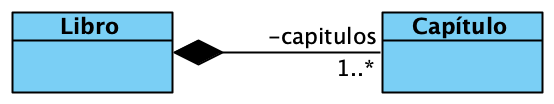
\includegraphics[ scale=.8]{analisisRequerimientos/clases/images/composicion}
						\caption{Ejemplo de composicion}
					}
					\label{fig:composicion}
				\end{center}
			\end{figure}
		}
		
	\end{itemize}
\end{itemize}

\subsection{Diagrama de clases del sistema}
La Figura \ref{fig:diagramaClases} muestra el diagrama de clases que fue definido para el desarrollo del proyecto.

\hypertarget{fig:diagramaClases}{
	\begin{figure}[htbp]
		\begin{center}
			\hypertarget{fig:diagramaClases}{
				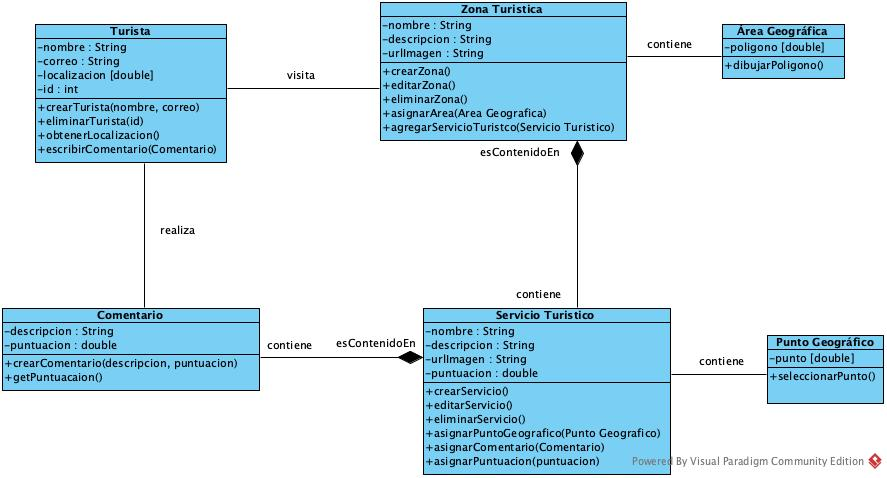
\includegraphics[ scale=.4]{analisisRequerimientos/clases/images/diagramaClases}
				\caption{Diagrama de clases del sistema}
			}
			\label{fig:diagramaClases}
		\end{center}
	\end{figure}
}